\section{CDS-Implied Italian Sovereign Default Intensities}
Conventions: quarterly payments ($\Delta=1/4$), premium is paid even in the default quarter, protection $(1-R)$ is paid at the end of the quarter of default, $R=40\%$. Discounting uses continuously compounded spot rates; for intermediate maturities we linearly interpolate spot rates between the provided $1,3,5,10$ year points and use $D(T)=e^{-r(T)T}$. Numerical results are computed from \texttt{data\_HW8.csv} in the accompanying notebook.
\subsection*{1(a)}
Let $\tau$ be the default time and let the (annual) risk-neutral default intensity be $\lambda$, so the default probability in any quarter is $\lambda/4$. Define $t_k=k/4$ and survival $S_k=\mathbb{P}(\tau>t_k)$. Then
\[
\mathbb{P}(\tau\le t_k)=1-S_k,\qquad S_k=(1-\lambda/4)^k.
\]
Since the buyer pays the premium at the end of quarter $k$ whenever it has survived to the start of that quarter, the expected present value (EPV) of premium payments on a 1-year CDS with annualized spread $S$ is
\[
\mathrm{PV}_{\text{prem}}(S;\lambda)=\sum_{k=1}^{4} e^{-r(t_k)t_k}\,\Big(\frac{S}{4}\Big)\,S_{k-1}.
\]
\subsection*{1(b)}
The probability that default occurs exactly in quarter $k$ is
\[
\mathbb{P}(t_{k-1}<\tau\le t_k)=S_{k-1}\,(\lambda/4).
\]
Thus the EPV of the protection leg is
\[
\mathrm{PV}_{\text{prot}}(\lambda)=\sum_{k=1}^{4} e^{-r(t_k)t_k}\,(1-R)\,S_{k-1}\,(\lambda/4).
\]
\subsection*{1(c)}
The fair spread $S$ solves $\mathrm{PV}_{\text{prem}}(S;\lambda)=\mathrm{PV}_{\text{prot}}(\lambda)$. Using
\[
\mathrm{PV}_{\text{prem}}(S;\lambda)=\sum_{k=1}^{4} e^{-r(t_k)t_k}\Big(\frac{S}{4}\Big)S_{k-1},
\qquad
\mathrm{PV}_{\text{prot}}(\lambda)=\sum_{k=1}^{4} e^{-r(t_k)t_k}(1-R)S_{k-1}\Big(\frac{\lambda}{4}\Big),
\]
we obtain
\[
\sum_{k=1}^{4} e^{-r(t_k)t_k}S_{k-1}\,\frac{S}{4}
=
\sum_{k=1}^{4} e^{-r(t_k)t_k}S_{k-1}\,(1-R)\frac{\lambda}{4}.
\]
Canceling the common factor $\sum_{k=1}^{4} e^{-r(t_k)t_k}S_{k-1}$ yields the closed form
\[
S=(1-R)\lambda.
\]
Hence, under the 1-year constant-intensity assumptions, $S$ does \emph{not} depend on the discount rates $\{r(t_k)\}$, and the implied intensity is
\[
\lambda=\frac{S}{1-R}.
\]
\paragraph{Example (first month in sample).} Using the July 2010 observation,
\[
\lambda_{1,2010\text{-}07}=0.017995.
\]
\subsection*{1(d)}
For a 3-year CDS, assume piecewise-constant intensities: $\lambda_1$ on $[0,1)$ and $\lambda_3$ on $[1,3)$. For quarter $k$, let $\lambda_k=\lambda_1$ if $t_{k-1}<1$ and $\lambda_k=\lambda_3$ otherwise. Then survival evolves as
\[
S_k=S_{k-1}\,(1-\lambda_k/4),\qquad S_0=1.
\]
The legs generalize to
\[
\mathrm{PV}_{\text{prem}}=\sum_{k=1}^{12} e^{-r(t_k)t_k}\,\Big(\frac{S}{4}\Big)\,S_{k-1},\qquad
\mathrm{PV}_{\text{prot}}=\sum_{k=1}^{12} e^{-r(t_k)t_k}\,(1-R)\,S_{k-1}\,(\lambda_k/4).
\]
Given the observed 1-year spread, we first solve for $\lambda_1$; then given the 3-year spread we solve for $\lambda_3$. For July 2010:
\[ \lambda_{3,2010\text{-}07} = 0.021785. \]
\subsection*{1(e)}
Assume $\lambda_3<\lambda_1$ and a constant discount rate $r$ (so $D(t_k)=e^{-rt_k}$). When $r$ increases, later cash flows are discounted more heavily. With $\lambda_3<\lambda_1$, default risk (and hence protection payments) is relatively front-loaded: a larger fraction of the protection leg occurs earlier than the premium leg, which continues (in expectation) into later quarters when the issuer survives. Increasing $r$ therefore reduces the present value of the (later-weighted) premium leg more than the protection leg, so the par spread $S$ must \emph{increase} to restore $\mathrm{PV}_{\text{prem}}=\mathrm{PV}_{\text{prot}}$.
\subsection*{1(f)}
With available 1-, 3-, 5-, and 10-year CDS spreads each month, we assume piecewise-constant intensities $\lambda_{1,t}$ on $[0,1)$, $\lambda_{3,t}$ on $[1,3)$, $\lambda_{5,t}$ on $[3,5)$, and $\lambda_{10,t}$ on $[5,10]$. For each month we bootstrap sequentially: solve $\lambda_{1,t}$ from the 1Y spread, then $\lambda_{3,t}$ from the 3Y spread given $\lambda_{1,t}$, then $\lambda_{5,t}$ from 5Y given prior, then $\lambda_{10,t}$ from 10Y.
\paragraph{Summary statistics (2010-07 to 2025-12).} The table reports the distribution of the monthly implied intensities:
\begin{table}[H]\centering
\begin{tabular}{lrrrr}\toprule
 & $\lambda_{1,t}$ & $\lambda_{3,t}$ & $\lambda_{5,t}$ & $\lambda_{10,t}$\\\midrule
mean & 0.012900 & 0.025768 & 0.035653 & 0.041790\\
std & 0.014952 & 0.018891 & 0.017413 & 0.011668\\
min & 0.000500 & 0.003777 & 0.008243 & 0.016646\\
25% & 0.004775 & 0.013916 & 0.024677 & 0.033617\\
50% & 0.008262 & 0.020406 & 0.031579 & 0.040105\\
75% & 0.014260 & 0.031192 & 0.042422 & 0.048106\\
max & 0.086352 & 0.101671 & 0.096597 & 0.085058\\
\bottomrule\end{tabular}
\end{table}
\paragraph{Time-series plot.} Figure~\ref{fig:lambdas} plots the four series together.
\begin{figure}[H]
\centering
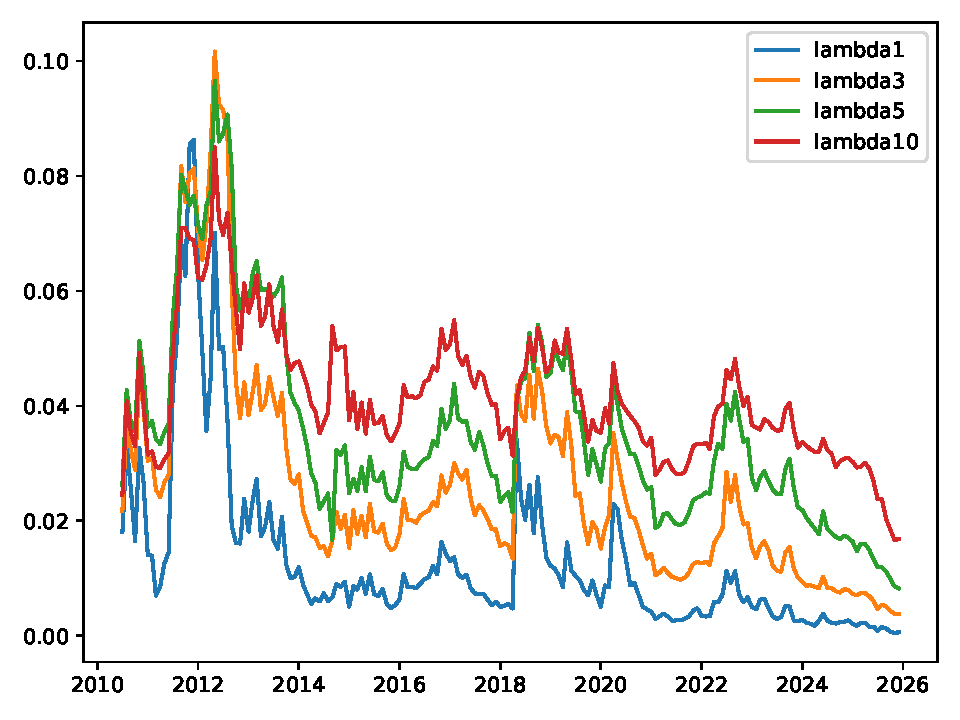
\includegraphics[width=0.9\textwidth]{./figures/ECO462_HW8_Q1_Model_1.pdf}
\caption{Monthly CDS-implied risk-neutral default intensities for Italy.}
\label{fig:lambdas}
\end{figure}
\paragraph{Comment on term structure.} Over most of the sample, the term structure is upward sloping: $\lambda_{1,t}<\lambda_{3,t}<\lambda_{5,t}<\lambda_{10,t}$. In the data, this monotone-increasing ordering holds about 88.9\% of months outside 2011--2012; the main alternative pattern is a mild hump where $\lambda_{5,t}>\lambda_{10,t}$ (about 10.5\% of those months).
\subsection*{1(g)}
In ``normal'' times (outside crisis periods), the typical ordering is $\lambda_{1,t}<\lambda_{3,t}<\lambda_{5,t}<\lambda_{10,t}$ (often with at most a mild hump at 5Y).
\paragraph{Eurozone crisis inversion check (2011--2012).} The months in 2011--2012 for which $\lambda_{1,t}>\lambda_{5,t}$ are:
\begin{table}[H]\centering
\begin{tabular}{lrrrr}\toprule
Month & $\lambda_{1,t}$ & $\lambda_{3,t}$ & $\lambda_{5,t}$ & $\lambda_{10,t}$\\\midrule
2011-11 & 0.085527 & 0.080517 & 0.075020 & 0.069134\\
2011-12 & 0.086352 & 0.081347 & 0.076603 & 0.068851\\
\bottomrule\end{tabular}
\end{table}
An inversion $\lambda_{1,t}>\lambda_{5,t}$ indicates that investors price especially high \emph{near-term} default risk relative to medium-term risk, consistent with acute rollover/liquidity concerns (e.g., fear of a near-term funding crisis) rather than a belief that the sovereign is fundamentally insolvent over the medium run. If CDS spreads spike but the ordering of $\lambda$ is preserved (still upward sloping), that pattern suggests investors are repricing default risk upward at all horizons but still view default risk as increasing with maturity; in the Italian context, this is consistent with elevated uncertainty but continued belief that fiscal adjustment/ECB backstops make the longer-run outlook less ``knife-edge'' than the short-run refinancing window.